\documentclass[12pt]{article}
\usepackage{vntex}
% \usepackage[english, vietnamese]{babel}
\usepackage{tikz}
\usepackage[left=2.00cm, right=2.00cm, top=3.50cm, bottom=2.00cm]{geometry}
\usepackage[unicode]{hyperref}
\usepackage{amsmath}
\usepackage{amssymb}
\usepackage{graphicx}
\usepackage{a4wide,amssymb,epsfig,latexsym,array,hhline,fancyhdr}
\usepackage[normalem]{ulem}
\usepackage[makeroom]{cancel}
\usepackage{amsthm}
\usepackage{multicol,longtable,amscd}
\usepackage{diagbox}
\usepackage{booktabs}
\usepackage{alltt}
\usepackage[framemethod=tikz]{mdframed}
\usepackage{caption,subcaption}
\usepackage{listings}
\usepackage{color}
\usepackage{lipsum}
\usepackage{setspace}
\usepackage{titling}
\usepackage{multicol}
\usepackage{indentfirst}
\usepackage{float}
\usepackage{fancyhdr}
\usepackage{scrextend}

\changefontsizes{13pt}

\pagestyle{fancy}

% \fontsize{14}{21}

\usetikzlibrary{decorations}
\usetikzlibrary{decorations.pathreplacing}
\usetikzlibrary{decorations.pathreplacing,calligraphy}
\usetikzlibrary{arrows.meta}
\usetikzlibrary{calc}

\setstretch{1.25}

\newtheorem*{theorem}{Định lý}
\newtheorem{corollary}{Hệ quả}
\newtheorem{lemma}{Bổ đề}
\newtheorem*{remark}{Nhận xét}
\newtheorem{definition}{Định nghĩa}
\newtheorem*{recap}{Tóm lại}


\title{}

\posttitle{
\par\end{center}
\begin{center}\LARGE(Toán rời rạc)\end{center}
\vskip0.5em}




\begin{document}
\fancyhf{}
\lhead{}
\chead{\thepage}
\rhead{}
\cfoot{}
\rfoot{}
\lfoot{}
\pagestyle{fancy}
% \addtolength{\topmargin}{-2.49998pt}
\renewcommand{\headrulewidth}{0pt}
\renewcommand{\footrulewidth}{0pt}
\begin{titlepage}
    \begin{center}
        ĐẠI HỌC QUỐC GIA HÀ NỘI \\
        \textbf{TRƯỜNG ĐẠI HỌC KHOA HỌC TỰ NHIÊN} \\
    \end{center}

    \vspace{1cm}

    \begin{figure}[h!]
        \begin{center}
            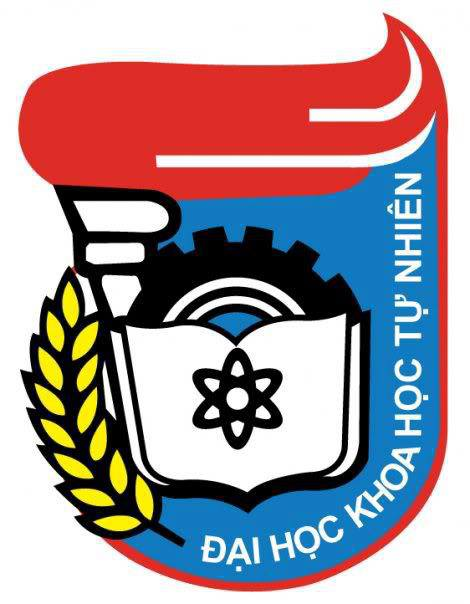
\includegraphics[width=4cm]{HUS.jpg}
        \end{center}
    \end{figure}

    \begin{center}
        \begin{tabular}{c}
            \multicolumn{1}{l}{\normalsize \textbf{TIỂU LUẬN HỌC PHẦN: LỊCH SỬ ĐẢNG CỘNG SẢN VIỆT NAM }} \\
            ~~                                                                                           \\
        \end{tabular}
        \begin{table}[H]
            \centering
            \begin{tabular}{rrl}
                \hspace{2cm} & \normalsize \textbf{HỌ VÀ TÊN:}    & \normalsize \textbf{NGUYỄN ĐỨC HUY} \\
                             & \normalsize \textbf{Mã sinh viên:} & \normalsize \textbf{19000350}       \\
            \end{tabular}
        \end{table}
    \end{center}
    \textbf{\large ĐỀ TÀI: ĐÁNH GIÁ QUAN ĐIỂM ĐỐI NGOẠI CỦA ĐẢNG CỘNG SẢN VIỆT NAM TẠI ĐẠI HỘI ĐẠI BIỂU TOÀN QUỐC LẦN THỨ XII (2016).}

    \vspace{1.5cm}
    \normalsize \centering Hà Nội, 2021
\end{titlepage}

\begin{titlepage}
    \tableofcontents
\end{titlepage}
\setcounter{page}{1}
\section{Mở đầu}
Đại hội XI (tháng 1/2011) đã có những bổ sung, phát triển phù hợp với tình
hình mới, từ đó chỉ rõ: ``Bảo đảm lợi ích quốc gia, giữ vững độc lập, tự chư, vì
hòa bình, hữu nghị, hợp tác và phát triển'', ``tôn trọng các nguyên tắc cơ bản
của luật pháp quốc tế, Hiến chương Liên hợp quốc''. Về phương châm, các văn kiện
của Đại hội khẳng định: Thực hiện nhất quán đường lối đổi ngoại độc lập, tự chủ,
hòa bình, hợp tác và phát triển; đa phương hóa, đa dạng hóa quan hệ, chủ động và
tích cực hội nhập quốc tế; là bạn, đối tác tin cậy và thành viên có trách nhiệm
trong cộng đồng quốc tế. Đổi mới trong đường lối đối ngoại của Việt Nam được đưa
ra tại đại hội XI là: Đánh dấu bước chuyển từ chủ động tích cực hội nhập kinh tế
quốc tế đến``chủđộng tích cực hội nhập quốc tế''. Đại hội cũng khẳng định cần
``triển khai đồng bộ toàn diện các hoạt động đối ngoại'', ``phối hợp hoạt động
đối ngoại của Đảng, ngoại giao Nhà nước và ngoại giao nhân dân, giữa ngoại giao
chính trị với ngoại giao kinh tế và ngoại giao văn hóa, giữa đối ngoại với quốc
phòng an ninh''.

Năm năm nhiệm kỳ đại hội Đảng lần thứ XII (2016 - 2021), là giai
đoạn chứng kiến sự sự thay đổi, sự rung chuyển và khó khăn mang tầm thế giới do
ảnh hưởng của đại dịch Covid 19. Những ảnh hưởng của đại dịch này đã đã thúc đẩy nhanh sự
chuyển biến đang diễn ra trước đây.

Đại hội XII của Đảng tiếp tục khẳng định
phương châm và định hướng lớn của hoạt động đối ngoại là ``Đa dạng hóa, đa phương
hóa trong quan hệ đối ngoại; chủ động và tích cực hội nhập quốc tế; là bạn, là
đối tác tin cậy và thành viên có trách nhiệm của cộng đồng quốc tế''. Đẩy mạnh và
làm sâu sắc hơn quan hệ với các đối tác, nhất là các đối tác chiến lược và các
nước lớn có vai trò quan trọng đối với phát triển và an sinh của đất nước, đưa
khuôn khổ quan hệ đã xác lập vào thực chất. Chủ động tham gia và phát huy vai trò
tại các cơ chế đa phương, đặc biệt là ASEAN và Liên hợp quốc. Chủ động, tích cực
tham gia các cơ chế đa phương về quốc phòng, an ninh\ldots Triển khai đồng bộ hoạt
động đối ngoại, cả về chính trị, an ninh, quốc phòng, kinh tế, văn hóa, xã hội.
Nâng cao chất lượng công tác tham mưu về đối ngoại và hội nhập quốc tế. Tăng
cường công tác thông tin đối ngoại, hội nhập quốc tế, tạo đồng thuận trong nước
và tranh thủ sự ủng hộ của bạn bè quốc tế đáp ứng yêu cầu xây dựng và bảo vệ đất
nước.

\section{Nội dung}
\subsection{Khái quát Đại hội XII của Đảng}
Đại hội đại biểu toàn quốc lần thứ XII Đảng Cộng
sản Việt Nam họp từ ngày 20-01-2016 đến ngày 28-01-2016, tại Thủ đô Hà
Nội, gồm 1.510 đại biểu thay mặt cho hơn 4,5 triệu đảng viên toàn
Đảng. Đại hội Tán thành những nội dung cơ bản về đánh giá tình
hình 5 năm thực hiện Nghị quyết Đại hội XI (2011 - 2015) và phương
hướng, nhiệm vụ 5 năm 2016 - 2020 nêu trong Báo cáo chính trị, Báo cáo kinh tế -
xã hội của Ban Chấp hành Trung ương Đảng khoá XI trình Đại hội;
Thông qua Báo cáo kiểm điểm sự lãnh đạo, chỉ đạo của Ban Chấp hành
Trung ương Đảng khoá XI trình Đại hội XII; Thông qua Báo cáo tổng
kết việc thi hành Điều lệ Đảng khoá XI; đồng ý không sửa đổi, bổ sung Điều lệ
Đảng hiện hành; Thông qua Báo cáo tổng kết thực hiện Nghị quyết Trung ương 4
khoá XI ``Một số vấn đề cấp bách về xây dựng Đảng hiện nay''; Thông qua kết
quả bầu Ban Chấp hành Trung ương Đảng khóa XII\@. Ban Chấp hành Trung ương
Đảng khóa XII và các cấp uỷ, tổ chức đảng lãnh đạo, chỉ đạo cụ thể
hoá và tổ chức thực hiện thắng lợi đường lối và những chủ trương nêu trong các
văn kiện Đại hội XII.

Tại đại hội Đảng lần thứ XII cũng đề ra phương
hướng cho mục tiêu 5 năm (2016 - 2021), đó là Tăng cường xây dựng Đảng trong
sạch, vững mạnh, nâng cao năng lực lãnh đạo và sức chiến đấu
của Đảng, xây dựng hệ thống chính trị vững mạnh. Phát huy sức mạnh
toàn dân tộc và dân chủ xã hội chủ nghĩa. Đẩy mạnh toàn diện,
đồng bộ công cuộc đổi mới; phát triển kinh tế nhanh, bền vững, phấn
đấu sớm đưa nước ta cơ bản trở thành nước công nghiệp theo hướng hiện đại.
Nâng cao đời sống vật chất và tinh thần của nhân dân. Kiên quyết, kiên trì
đấu tranh bảo vệ vững chắc độc lập, chủ quyền, thống nhất, toàn vẹn lãnh
thổ của Tổ quốc, bảo vệ Đảng, Nhà nước, nhân dân và chế độ xã hội
chủ nghĩa. Giữ gìn hoà bình, ổn định, chủ động và tích cực hội nhập
quốc tế để phát triển đất nước; nâng cao vị thế và uy tín của Việt Nam trong khu
vực và trên thế giới. Trong đó đặc biệt nhấn mạnh về đường lối đối
ngoại của dân tộc ta trong giai đoạn mới: ``Thực
hiện nhất quán đường lối đối ngoại độc lập, tự chủ, hòa bình, hợp
tác và phát triển, Đa dạng hóa, đa phương hóa trong quan hệ đối
ngoại; chủ động và tích cực hội nhập quốc tế; là bạn, là
đối tác tin cậy và thành viên có trách nhiệm của cộng đồng quốc tế''. Đây
được xem là bước hoàn thiện trong chủ trương đổi mới, mở cửa đất nước được đề ra
tại Đại hội Đảng lần thứ VI của Đảng, được nhấn
mạnh, phát triển theo từng Đại Hội tiếp theo, tùy thuộc
vào hoàn cảnh thực tế mà đưa ra mục tiêu khác nhau. Nhưng tựu chung vẫn là: Đưa
Việt Nam mở cửa, hội nhập nhằm tận dụng thời cơ trong bối cảnh toàn
cầu hóa, phát triển đất nước về mọi mặt, nhưng vẫn giữ được bản sắc dân
tộc.

\subsection{Giải thích một số khái niệm trong quan điểm đối ngoại của Đảng tại đại hội XII}
Trước hết, để đánh giá được chủ chương ``Thực hiện nhất quán đường lối đối
ngoại độc lập, tự chủ, hòa bình, hợp tác và phát triển, đa
dạng hóa, đa phương hóa trong quan hệ đối ngoại; chủ động và
tích cực hội nhập quốc tế; là bạn, là đối tác tin cậy và thành viên
có trách nhiệm của cộng đồng quốc tế''. Ta cần làm rõ một số
khái niệm sau đây:

Đối ngoại là tiến hành trong việc đàm phán, dàn xếp thương lượng giữa
những người đại diện cho một nhóm hay một quốc gia.

Đa dạng hóa các quan hệ đối ngoại là làm cho hoạt động
đối ngoại trở nên đa dạng hơn, quan hệ trên nhiều mặt, nhiều phương
diện về kinh tế chính trị xã hội.

Đa phương hóa các quan hệ đối ngoại là việc thực hiện đối ngoại với
nhiều bên cùng một lúc, nói cách khác là quan hệ đối ngoại có sự
thỏa thuận hay tham gia của nhiều bên.

Với quan điểm Đại Hội lần thứ XII của Đảng cho thấy: Đảng ta
xây dựng đường lối đối ngoại với phương châm, mở cửa đất nước, tăng
cường sự giao lưu hợp tác giữa các quốc gia và vùng lãnh thổ trên thế giới, tích
cực tham gia vào các tổ chức quốc tế, tăng cường hội nhập kinh tế quốc tế,
dựa trên sự hòa bình, hợp tác cùng phát triển, trên cơ sở tôn trọng hòa bình,
độc lập dân tộc, tự chủ của các nước, du trong hoàn cảnh nào, Việt
Nam cũng phải là một quốc gia độc lập, tự chủ và có quyền tự
quyết mọi vấn đề nội tại của đất nước mà không chịu sự chi phối của
bất cứ một quốc gia hay tổ chức nào.
\subsection{Đánh giá quan điểm ``Thực hiện nhất quán đường lối đối ngoại độc lập, tự chủ,
    hòa bình, hợp tác và phát triển, đa dạng hóa, đa phương hóa trong quan hệ đối
    ngoại; chủ động và tích cực hội nhập quốc tế; là bạn, là đối tác tin cậy và
    thành viên có trách nhiệm của cộng đồng quốc tế''}

Trước hết, phải khẳng định, quan điểm đối ngoại của Đảng là ``Thực
hiện nhất quán đường lối đối ngoại độc lập, tự chủ, hòa bình,
hợp tác và phát triển, đa dạng hóa, đa phương hóa trong quan hệ đối
ngoại; chủ động và tích cực hội nhập quốc tế; là bạn,
là đối tác tin cậy và thành viên có trách nhiệm của cộng đồng quốc
tế'' là hoàn toàn đúng đắn và có tính tất yếu trong bối cảnh hiện nay khi mà
công nghệ - khoa học kĩ thuật, đặc biệt là internet đã đập tan mọi khoảng
cách, giới hạn về vị trí địa lý, giúp cho con người ở những nơi xa
lạ tiến đến gần nhau hơn. Trải qua thời kỳ cách mạng 4.0,
đã giúp thay đổi bộ mặt thế giới. Mặt khác, cuộc khủng hoảng d
đại dịch Covid 19 đã tạo ra một bước rung chuyển chưa từng
có từ sau chiến tranh thế giới thứ 2. Điều này đòi hỏi, các nước
cần phải có những bước đi đúng đắn để vừa có thể giải quyết các vấn đề
về dịch bệnh, đi đôi với giữ gìn và phát triển kinh tế, xây dựng hệ thống
chính trị, văn hóa xã hội để củng cố chính quyền, đảm bảo an ninh quốc
phòng. Mặt khác, Đất nước ta đã trải qua 30 năm đổi mới, Đất nước ta đã đã
mở rộng và đưa vào chiều sâu quan hệ với tất cả các đối tác và
đạt được nhiều thành tựu, Tuy nhiên, quá trình triển khai định hướng
này còn có những tồn tại. Cụ thể như sau:
\subsubsection{Về Thành Tựu}
\textit{Về kinh tế}: Kinh tế nước ta duy trì được tốc độ tăng trưởng bình quân khá
cao (khoảng 5,9\%). Nhiều khó khăn, vướng mắc, hạn chế, yếu kém từ
các năm trước đã được tập trung giải quyết và đạt những kết quả bước
đầu. Chất lượng tăng trưởng được cải thiện; kinh tế vĩ mô ổn định khá vững
chắc; lạm phát được kiểm soát và duy trì ở mức thấp; các cân đối lớn của
nền kinh tế tiếp tục được bảo đảm và có bước được cải thiện; kỷ luật, kỷ
cương tài chính - ngân sách nhà nước được tăng cường. Huy động vốn
đầu tư toàn xã hội tăng mạnh, hiệu quả sử dụng được nâng lên.
Cán cân thương mại được cải thiện; xuất khẩu tăng nhanh. Cơ cấu lại
nền kinh tế gắn với đổi mới mô hình tăng trưởng, thực hiện ba đột phá
chiến lược đạt được những kết quả quan trọng. Môi trường đầu tư,
kinh doanh, tiềm lực, quy mô và sức cạnh tranh của nền kinh tế tiếp tục
được nâng lên. Chính trị, xã hội ổn định, đời sống của nhân dân được cải
thiện rõ rệt. Các lĩnh vực an sinh xã hội, y tế, giáo dục-đào tạo,
khoa học-công nghệ, bảo vệ môi trường, phát triển văn hoá, xây dựng con người
Việt Nam, v.v\ldots có nhiều chuyển biến tích cực, có mặt khá nổi bật. Năm 2020,
trong bối cảnh đại dịch Covid 19 tác động mạnh.trong khi kinh
tế thế giới suy thoái, tăng trưởng âm gần 4\%, kinh tế nước ta vẫn
đạt mức tăng trưởng 2,91\%, là một trong những nền kinh tế có tốc
độ tăng trưởng cao nhất thế giới.

\textit{Về hợp tác song phương}: Nước ta tăng cường mối quan hệ hợp tác với các nước láng
giềng, các nước chung biên giới, trong khu vực và trên thế giới, tăng cường
hợp tác có chiều sâu, xây dựng mối quan hệ hợp tác bền vững và ổn định, mở
rộng đối tác chiến lược. Trong giai đoạn này, ta đã thiết lập quan
hệ đối tác toàn diện với 5 nước, nâng cấp qua hệ đối tác chiến lược với 2 nước
(Australia năm 2018 và New Zealand 2020), thay đổi từ đối tác chiến lược lên đối
tác chiến lược toàn diện với Ấn Độ vào năm 2016, nâng tổng số quan hệ đối
tác chiến lược toàn diện lên 30 nước.

\textit{Về hợp tác đa phương}: Gia nhập và trở thành một ``mắt xích'' quan trọng
trong mạng lưới các liên kết kinh tế với các nền kinh tế hàng
đầu thế giới. Chúng ta đã là thành viên chính thức của ASEAN, APEC, ASEM
và WTO cũng như nhiều định chế tài chính như WB, ADB, IMF\ldots Việc gia
nhập WTO vào năm 2007 đã mở ra quan hệ thương mại bình đẳng giữa Việt Nam
với 150 quốc gia và vùng lãnh thổ. Đây là một thành tựu quan trọng của
việc thực hiện chính sách đối ngoại đổi mới, đưa Việt Nam trở thành quốc
gia bình đẳng trong thương mại với các nước trên thế giới. Việt Nam ngày
càng nâng tầm hiệu quả vai trò đối ngoại đa phương, tích cực đóng
góp xây dựng, định hình các thể chế đa phương, từng bước phát huy vai trò hòa
giải, góp phần vào hòa bình và ổn định khu vực.

\textit{Về Văn hóa xã hội}: Công tác ngoại giao văn hóa đã góp phần
quảng bá và nâng tầm hình ảnh của Việt nam đến bạn bè quốc tế,
nâng cao tình hữu nghị giữa các nước, thay đổi nhận thức của thế giới về văn hóa,
truyền thống con người Việt Nam, tránh những xuyên tạc sai lệch của các
thế lực thù địch. Giai đoạn 2016 - 2020, Nước ta đã tăng tổng giá trị di sản
được UNESCO công nhận lên 39 di sản, qua đó tạo nguồn lực cho sự phát
triển kinh tế - xã hội.

\textit{Về an ninh quốc phòng}: Công tác an ninh quốc phòng được giữ vững,phối hợp
triển khai có hiệu quả trong công cuộc bảo vệ biên giới và cửa khẩu, ký
kết các văn kiện , thỏa thuận về biên giới với trung quốc, lào và
campuchia. Tình hình biển đông dù diễn biến phức tạp, ta vẫn kiên quyết,
kiên trì đấu tranh, bảo vệ chủ quyền biển đảo, Tích cực đàm phán giải quyết các
tranh chấp, khác biệt liên quan đến vùng kinh tế đối tác với Malaysia,Indonesia.
Đặc biệt, trong đại dịch Covid 19, ta tích cực đàm phán, tổ chức các
chuyến bay giải cứu, đón kiều bào của ta ở nước ngoài về nước, với phương châm
``Không một ai bị bỏ lại phía sau''. Kịp thời xử lý các vấn đề liên
quan đến công dân của ta ở nước ngoài.

\subsubsection{Hạn chế}
Dù đạt được nhiều thành tựu to lớn, nhưng đường lối đối ngoại của Đảng trong giai
đoạn này vẫn còn nhiều hạn chế, đó là:

Thứ nhất, thời gian qua trong một số vấn đề, ở một số thời điểm nhận
thức của chúng ta không theo kịp tình hình. Chúng ta đã không lường hết được
những diễn biến phức tạp, nhanh chóng trong chính sách và quan hệ của các
nước lớn, nhất là của Mỹ và quan hệ Mỹ - Trung. Nguyên nhân của tình trạng
này chủ yếu là do các yếu tố khách quan, do tình hình thế giới, khu vực biến
động rất phức tạp, khó lường. Nhưng công tác nghiên cứu đánh giá
tình hình và dự báo chiến lược vẫn chưa được như mong muốn

Thứ hai, việc triển khai đường lối và chính sách đối ngoại trong thực tiễn
vẫn chưa mạnh mẽ, đồng bộ và toàn diện. Việc tạo đan xen
lợi ích, đưa quan hệ đi vào chiều sâu, xây dựng các khuôn khổ quan hệ thực chất
và hiệu quả, triển khai các thỏa thuận đã ký kết thực chất, tham gia và
tận dụng các thể chế đa phương, nhất là ASEAN để bảo vệ tốt hơn lợi ích của Việt
Nam vẫn còn chưa được như mong muốn. Sự tham gia của các bộ ngành và địa
phương vào công tác đối ngoại còn chưa đồng đều.

\subsubsection{Cơ hội và thách thức}
\textit{Về cơ hội}:

Nền kinh tế Việt Nam có tốc độ tăng trưởng nhanh, những
kinh nghiệm trong quá trình hội nhập sẽ tạo động lực cho kinh
tế nước ta phát triển. mắt khác, chúng ta nằm ở vị trí địa lý lý chiến lược của
khu vực châu á - Thái Bình Dương, đây được xem là khu vực năng động, là
nhanatoso quan trọng trong chính sách phát triển của các nước. Thêm vào đó., Ta
có sự lãnh đạo sáng suốt của Đảng, Với sự vào cuộc của toàn bộ
hệ thống chính trị, với nền tảng là con người là chủ đạo.

\textit{Về thách thức}:

Cục diện thế giới tiếp tục biến đổi theo xu hướng đa cực, đa
trung tâm, và đấu tranh vẫn song hành, kiềm chế lẫn nhau đang ngày càng trở nên
gay gắt, đặc biệt là sự trỗi dậy của chủ nghĩa dân tộc. Luật pháp quốc tế
còn nhiều hạn chế. Kinh tế khủng hoảng, suy thoái do đại dịch Covid
19 kéo dài. Khu vực Châu Á Thái Bình Dương cạnh tranh ngày càng gay gắt,
đặc biệt là tranh chấp chủ quyền lãnh thổ, chủ quyền biển đảo ngày càng phức
tạp.

Trong khi đó, Việt nam đối diện với những thách thức nội
tại, nền kinh tế phát triển chưa bền vững lại chịu tác động
của đại dịch Covid 19. Xu hướng già hóa dân số nhanh, năng lực
cạnh tranh của các doanh nghiệp Việt còn chưa cao, công tác dự báo chiến
lược còn chưa chủ động, nhạy bén.

\subsubsection{Đề xuất một số giải pháp}
Nhằm phát huy tối đa những lợi thế, khắc phục những hạn chế về đường lối
đối ngoại trong thời kỳ mới, cần phải thực hiện một số
biện pháp sau đây:

Nhận thức sâu sắc về thời cơ, thách thức mà hội đối
ngoại đa phương mang lại. Nâng cao năng lực cạnh tranh, không
ngừng đổi mới, sáng tạo công nghệ. Hoàn Thiện thể chế kinh tế và luật pháp.
Xây dựng chiến lược và lộ trình hội nhập - phù hợp. Xây dựng nền
kinh tế độc lập tự chủ của Việt Nam.

\section{Lời kết}
Quan điểm ``Thực hiện nhất quán đường lối đối ngoại độc lập, tự chủ,
hòa bình, hợp tác và phát triển, đa dạng hóa, đa phương hóa trong quan
hệ đối ngoại; chủ động và tích cực hội nhập quốc tế; là
bạn, là đối tác tin cậy và thành viên có trách nhiệm của cộng đồng
quốc tế'' là hoàn toàn đúng đắn, phù hợp với bối cảnh thế giới , là sự hoàn
thiện có tính tất yếu mang tính lịch sử. Việt Nam đang bước vào thời kỳ mới với
thế và lực mới do những thành tựu và kinh nghiệm 30 năm đổi mới mang lại, với vị
thế ngày càng nâng cao trên trường quốc tế, cơ hội rất lớn và thách thức cũng
không nhỏ.

Đường lối đối ngoại đổi mới của Đảng qua các kỳ Đại hội nhất
là Đại hội XII đã thể hiện sự nhất quán, sáng tạo và hệ
thống với tầm cao mới. Chúng ta tin tưởng rằng, với kinh nghiệm lãnh
đạo cách mạng của Đảng và đặc biệt trong 30 năm đổi mới toàn diện
đất nước theo định hướng xã hội chủ nghĩa sẽ phát huy sức mạnh tổng
hợp để đưa sự nghiệp cách mạng nước ta sang một bước ngoặt mới. Thực
hiện đường lối đối ngoại đúng đắn của Đảng, trong thời gian tới hoạt
động đối ngoại và hội nhập quốc tế của nước ta sẽ đạt
được nhiều thành tựu to lớn, giữ vững môi trường hòa bình và phát huy
ngoại lực sớm đưa nước ta trở thành nước công nghiệp theo hướng hiện
đại; thực hiện thắng lợi mục tiêu dân giàu, nước mạnh, dân chủ, công
bằng, văn minh.

\begin{thebibliography}{9}
    \bibitem{latexcompanion}
    Đảng Cộng sản Việt Nam.
    \textit{Văn kiện Đại hội đại biểu toàn quốc lần thứ XI}. \\
    NXB. Chính trị quốc gia – Sự thật, Hà Nội, 2011.

    \bibitem{latexcompanion}
    Đảng Cộng sản Việt Nam.
    \textit{Văn kiện Đại hội đại biểu toàn quốc lần thứ XII}. \\
    Văn phòng Trung ương Đảng, Hà Nội, 2016.


\end{thebibliography}

\end{document}